\documentclass[a4paper]{article}
\usepackage{geometry}
\geometry{
	a4paper,
	total={170mm,257mm},
	left=27mm,
	right=30mm,
	top=30mm,
	bottom= 30mm
}
\usepackage{lipsum}
\usepackage{tabu}
\usepackage[english]{babel}
\usepackage[utf8]{inputenc}
\usepackage[parfill]{parskip}
\usepackage{longtable}
\usepackage{amsmath}
\usepackage{graphicx}
\usepackage{enumitem}
\usepackage[colorinlistoftodos]{todonotes}
\usepackage{tikz}
\newcommand*\circled[1]{\tikz[baseline=(char.base)]{
		\node[shape=circle,draw,inner sep=0.5pt] (char) {#1};}}
\usetikzlibrary{fit,positioning}
\usepackage{authblk}
\usepackage{natbib}
\usepackage[algo2e]{algorithm2e}
\usepackage{algorithmic}  
\usepackage{algorithm}
\usepackage{comment}
\usepackage{bbm}
\usepackage{array}% http://ctan.org/pkg/array
\makeatletter
\g@addto@macro{\endtabular}{\rowfont{}}% Clear row font
\makeatother
\newcommand{\rowfonttype}{}% Current row font
\newcommand{\rowfont}[1]{% Set current row font
	\gdef\rowfonttype{#1}#1%
}
\newcolumntype{L}{>{\rowfonttype}l}
\title{Getting It Right for the IPTM}

\author[1]{Bomin Kim}
\author[3]{Aaron Schein}
\author[1]{Bruce Desmarais}
\author[2,3]{Hanna Wallach}
\affil[1]{Pennsylvania State University}
\affil[2]{Microsoft Research NYC}
\affil[3]{University of Massachusetts Amherst}

\begin{document}
\setlength{\parindent}{0pt}
\maketitle
\begin{abstract}
	
	\noindent Software development is integral to the objective of applying the IPTM ---the interaction-partitioned topic model--- to real world data. Code review is a valuable process in any research computing context, and the prevalence of software bugs in statistical software is well documented \citep[e.g., ][]{altman2004numerical,mccullough2009accuracy}.  With highly complex models such as the IPTM, there are many ways in which software bugs can be introduced and go unnoticed. As such, we present a joint analysis of the integrity of our generative model, sampling equations, and software implementation for the IPTM. ``Getting it Right" \citep{geweke2004getting} test is very simple to implement, yet very powerful because it amplifies subtle
	misktakes, either in the sampling equations or code. We hope that all researchers should be using GiR whenever they derive and implement Markov Chain Monte Carlo (MCMC) inference for a Bayesian latent variable model.
\end{abstract}
  \section{Getting It Right (GiR) Test}
 \cite{geweke2004getting} introduced the ``Getting it Right'' (GiR) test---a joint distribution test of posterior simulators which can detect errors in sampling equations as well as coding errors.  The test involves comparing the distributions of variables simulated from two joint distribution samplers, which we call ``forward" and ``backward" samples. The forward sampler draws unobservable variables from the prior and then generates the observable data conditional on the unobservables. The backward sampler alternates between the inference and an observables simulator, by running the inference code on observable data to obtain posterior estimates of the unobervable variables and then re-generating the observables given the inferred unobservables. The backward sampler is initialized by running an iteration of inference on observables drawn directly from the prior. Since the only information on which both the forward and backward samplers are based is the prior, if the sampling equations are correct and the code is implemented without bugs, each variable should have the same distribution in the forward and backward samples. In other words, if there are no mistakes, then the
 forward samples and the backward samples should be indistinguishable.

  \subsection{IPTM: Forward Generating Process} \label{subsec: Forward Generative Process}
In order to draw forward samples, we first draw all unobservable variables, \textit{e.g.} $\boldsymbol{\phi}, \boldsymbol{\theta}, \boldsymbol{l}, \boldsymbol{b}, \boldsymbol{\eta}, \delta$, from their respecitve prior distributions and then generates the observable data, \textit{e.g.} $\boldsymbol{w}, \boldsymbol{a}, \boldsymbol{r}, \boldsymbol{t}$, conditional on the generated latent variables. The forward generating process of the IPTM exactly follows Section 2 in the main paper, summarized in Algorithm \ref{alg:forward} below.
  	\begin{algorithm}[H]
  		\SetAlgoLined
  		\caption{Forward Generating Process}
  			Input:\\
  			1. Number of classes, \textit{e.g.} $D$ (documents), $V$ (words), $K$ (topics), $\{N_d\}_{d=1}^D$ (tokens), $A$ (actors), and $C$ (interaction patterns)\\
  			2. Timestamp distribution and link function, \textit{e.g.} lognormal with identity link\\ 
 			3. Hyperparameters, \textit{e.g.} $\alpha, \beta, \boldsymbol{m}, \boldsymbol{\mu}_b, \Sigma_b, \boldsymbol{\mu}_\eta, \Sigma_\eta, \mu_\delta, \sigma^2_\delta$ and $(a_\tau, b_\tau)$ if $\sigma_\tau^2$ needed.\\
 			
 			\textbf{Unobservables from prior distributions}
	  		\begin{itemize}
	  			\item For $k=1,\ldots, K$
	  			\begin{itemize}
	  			\item[-] $\boldsymbol{\phi}_k \sim \mbox{Dirichlet}\Big(\beta, (\frac{1}{V},\ldots,\frac{1}{V})\Big)$
	  			\item[-] $l_k\sim \mbox{Uniform}(1, C)$
	  			\end{itemize}
	  			\item For $d=1,\ldots, D,$
	  			\begin{itemize}
	  			\item[-] $\boldsymbol{\theta}_d \sim \mbox{Dirichlet}\Big(\alpha, (m_1,\ldots,m_K)\Big)$
	  			\end{itemize}
	  			\item For $c=1,\ldots, C$
	  			\begin{itemize}
	  				\item[-] $\boldsymbol{b}_c \sim \mbox{Normal}(\boldsymbol{\mu}_b,  \Sigma_b)$
	  				\item[-] $\boldsymbol{\eta}_c \sim \mbox{Normal}(\boldsymbol{\mu}_\eta,  \Sigma_\eta)$
	  			\end{itemize}
	  			\item $\delta \sim \mbox{Normal}(\mu_\delta, \sigma^2_\delta)$ 
	  			\item $\sigma_\tau^2 \sim \mbox{Inverse-Gamma}(a_\tau, b_\tau)$\\
	  		\end{itemize}
	  		
	  	\textbf{Observables from generative process}\\
  		\For{d=1 to D}{
  			\For{n=1 to ${N}_d$}{
  				draw $z_{dn} \sim \mbox{Multinomial}(\boldsymbol{\theta}_d))$\\
  				draw $w_{dn} \sim\mbox{Multinomial} (\phi_{z_{dn}})$
  			}
  			\For{c=1 to $C$}{
  				set $\pi_{dc} =  \frac{\sum_{k:l_k=c}N_{dk}}{N_d}$
  			}
  			\For{i=1 to $A$}{
  				\For {j = 1 to $A$}{
  				calculate $\boldsymbol{\nu}_{idjc}=\{\nu_{idjc}\}_{c=1}^C$, where $\nu_{idjc}= \mbox{exp}\Big({\boldsymbol{b}_c}^{\top}\boldsymbol{x}_{idjc}\Big)$\\ calculate $\lambda_{idj} =\sum_{c=1}^{C} \pi_{dc}\, \nu_{idjc}$,
  				}
  				draw $\boldsymbol{u}_{id}  \sim
  				\mbox{Gibbs}(\delta, \boldsymbol{\lambda}_{id})$\\
  				calculate $\boldsymbol{\xi}_{idc}=\{\xi_{idc}\}_{c=1}^C$, where $\xi_{idc}= \boldsymbol{\eta}_c^\top\mbox{GeomMean}(\{ \boldsymbol{y}_{idjc}\}_{j:u_{idj}= 1})$\\
  				calculate $\mu_{id} = \sum_{c=1}^C \pi_{dc} g^{-1}(\xi_{idc})$\\
  				draw $\tau_{id} \sim \phi_\tau(\mu_{id}, \sigma^2_\tau),$ where $\phi_\tau$ is the pdf of specified timestamp distribution 
  			}
  				set $a_d = \mbox{argmin}_{i}(\tau_{id})$,
  				$\boldsymbol{r}_d = \boldsymbol{u}_{a_d d},$ and
  				$t_d =t_{d-1} + \tau_{a_d d}$.
  			}
  			\label{alg:forward}
  		\end{algorithm}
  		   
 \subsection{IPTM: Backward Generating Process} \label{subsec: Backward Generative Process}
                  Next, we take one of these
                  forward samples and, given this sample, draw a sample of the latent
                  variables from their posterior distribution using our inference
                  code. We then use the final step of the generative process to draw a
                  new sample of the data given this sample of the latent
                  variables. Finally, we repeat the last two steps many times to
                  obtain a set of backward samples. 
                  
                  For backward sampling, we let $N_{vk}$ be the number of tokens of word-type $v$ that are currently assigned to topic $k$. Also let $N_k$ be the total number of tokens currently assigned to topic $k$. Word-assignments are implemented via collapsed Gibbs sampling \citep{griffiths2002gibbs}, while the generation of tie data $(a_d, \boldsymbol{r}_d, t_d)$ directly follows the generating process, same as the forward generating process. This ``backward" version of the generative process is illustrated in Algorithm \ref{alg:backward} below.
                  \begin{algorithm}[H]
                  	\SetAlgoLined
                  	\caption{Backward Generating Process}
                  	Input:\\
                  	1. One set of forward sample\\
                  	2. Inference setting, \textit{e.g.} number of outer iterations, length of Metropolis-Hastings (M-H) chains\\ 
                  	3. Timestamp distribution and link function, \textit{e.g.} lognormal with identity link\\ 
                  	
                  	\textbf{Inference on one forward sample}\\
                  	\For{o = 1 to O}{
                  			Run inference code according to Algorithm 1 in IPTM paper (see Section 3)\\
                  			(NOTE: ensure full convergence on all latent variables)
                  		}
                  	\vspace{4mm}              	             
                  	\textbf{Unobservables from inference}
                  	\begin{itemize}
                  		\item For $k=1,\ldots, K$
                  		\begin{itemize}
                  			\item[-] obtain the last of $l_k$
                  		\end{itemize}
                  		\item For $d=1,\ldots, D,$
                  		\begin{itemize}
                  			\item[-] obtain the last sample of $\boldsymbol{z}_d$ 
                  		\end{itemize}
                  		\item For $c=1,\ldots, C$
                  		\begin{itemize}
                  			\item[-] obtain the posterior mean of $\boldsymbol{b}_c$ 
                  			\item[-] obtain the posterior mean of $\boldsymbol{\eta}_c$ 
                  		\end{itemize}
                  		\item obtain the posterior mean of $\delta$ 
                  		\item  obtain the posterior mean of $\sigma_\tau^2$,
                  	\end{itemize}
                  		where the posterior means are calculated from MCMC chains via M-H. \\
                  		
                  	\textbf{Observables from generative process}\\
                  	set all $N_{vk}= 0$ and $N_k = 0$\\
                  	\For{d=1 to D}{
                  		\For{n=1 to $ {N}_d$}{
                  			\For{v=1 to $V$}{
                  				$\mbox{token-word-type-distribution}_{dn}[v] = \frac{N_{ z_{dn}v}+\beta/V}{N_{z_{dn}} + \beta}$
                  			}
                  			draw $w_{dn} \sim (\mbox{token-word-type-distribution}_{dn})$\\
                  			$N_{w_{dn}, z_{dn}} += 1$\\
                  			$N_{z_{dn}} += 1$
                  		}
                  		\For{c=1 to $C$}{
                  			set $\pi_{dc} =  \frac{\sum_{k:l_k=c}N_{dk}}{N_d}$
                  		}
                  		\For{i=1 to $A$}{
                  			\For {j = 1 to $A$}{
                  				calculate $\boldsymbol{\nu}_{idjc}=\{\nu_{idjc}\}_{c=1}^C$, where $\nu_{idjc}= \mbox{exp}\Big({\boldsymbol{b}_c}^{\top}\boldsymbol{x}_{idjc}\Big)$\\ calculate $\lambda_{idj} =\sum_{c=1}^{C} \pi_{dc}\, \nu_{idjc}$,
                  			}
                  			draw $\boldsymbol{u}_{id}  \sim
                  			\mbox{Gibbs}(\delta, \boldsymbol{\lambda}_{id})$\\
                  			calculate $\boldsymbol{\xi}_{idc}=\{\xi_{idc}\}_{c=1}^C$, where $\xi_{idc}= \boldsymbol{\eta}_c^\top\mbox{GeomMean}(\{ \boldsymbol{y}_{idjc}\}_{j:u_{idj}= 1})$\\
                  			calculate $\mu_{id} = \sum_{c=1}^C \pi_{dc} g^{-1}(\xi_{idc})$\\
                  			draw $\tau_{id} \sim \phi_\tau(\mu_{id}, \sigma^2_\tau),$ where $\phi_\tau$ is the pdf of specified timestamp distribution 
                  		}
                  		set $a_d = \mbox{argmin}_{i}(\tau_{id})$,
                  		$\boldsymbol{r}_d = \boldsymbol{u}_{a_d d},$ and
                  		$t_d =t_{d-1} + \tau_{a_d d}$.
                  	}
                  	\label{alg:backward}
                  \end{algorithm}
        
\section{Statistics to Use}
To compare the forward and backward samples, we need some discrepancy functions that measure important properties of generated data. It is recommended to specify various statistics such that we can not only compare the observables (\textit{i.e.} generated data), but also compare the unobservables (\textit{i.e.} latent variables).  For each forward and backward sample from the IPTM that consists of $D$ number of documents, we save the statistics below.
      \begin{itemize}
      	\item[1.] Mean of interaciton-pattern-specific recipient coefficients $(\boldsymbol{b}_1,\ldots,\boldsymbol{b}_C)$,
      	\item[2.] Mean of interaciton-pattern-specific timestamp coefficients $(\boldsymbol{\eta}_1,\ldots,\boldsymbol{\eta}_C)$,
      	\item[3.] Recipient size parameter $\delta$ value used to generate forward/backward samples
      	\item[4.] Timestamp variance parameter $\sigma_\tau^2$ used to generate the samples
        \item[5.] Mean of the observed recipient size $ \lVert\boldsymbol{r}_d\rVert_1 $ across $d=1,...,D$,
      	\item[6.] Mean of time-increments $t_d-t_{d-1}$ across $d=1,...,D$,
      	\item[7.] Mean topic-interaction pattern assignment $l_k$ across $k=1,...,K$, 
      	\item[8.] Number of tokens in topics assigned to each interaction pattern $c=1,...,C$,
      	\item[9.] Number of tokens assigned to each topic $k=1,...,K$, 
       \item[10.] Number of tokens assigned to each unique word type $w=1,...,W$,
      	 \end{itemize}
where the statistics 1--4 directly measure the unobservables, while the rest 5--10 examine some features of the observed data.
\section{Results}
To keep the computational burden of re-running thousands of rounds of inference manageable, we ran the GiR using a relatively small artificial sample, consisting of 5 documents, 4 tokens per document, 4 actors, 5 unique word types, 2 interaction patterns, and 4 topics per each forward or backward samples. For detailed settings including the prior specifications, see Appendix \ref{subsec: GiR implementation}.
We generated $10^5$ sets of forward and backward samples, and then calculated 1,000 quantiles for each of the coefficients, $\boldsymbol{b}$ and $\boldsymbol{\eta}$, and 50 quantiles for the rest of the statistics. We also calculated t-test and Mann-Whitney test p-values in order to test for differences in the distributions generated in the forward and backward samples. Before we calculated these statistics, we thinned our samples by taking every 9th sample starting at the 10,000th sample for a resulting sample size of 10,000, in order to reduce the autocorrelation in the Markov chains. In each case, if we observe a large p-value, this gives us evidence that the distributions generated under forward and backward sampling have the same locations. 

We depict the GiR results using probability-probability (PP) plots. To compare two samples with a PP-plot we calculate the empirical quantile in each sample of a set of values observed across the two samples, then plot the sets of quantiles in the two samples against each other. If the two samples are from equivalent distributions, the quantiles should line up on a line with zero $y$-intercept, and unit slope (\textit{i.e.} a 45-degree line). Figure \ref{fig:PPplot2} presents our results. All the blue dots lie on the
45-degree red line, so our derivations and code pass the test.
\begin{figure}[H]
	\centering
	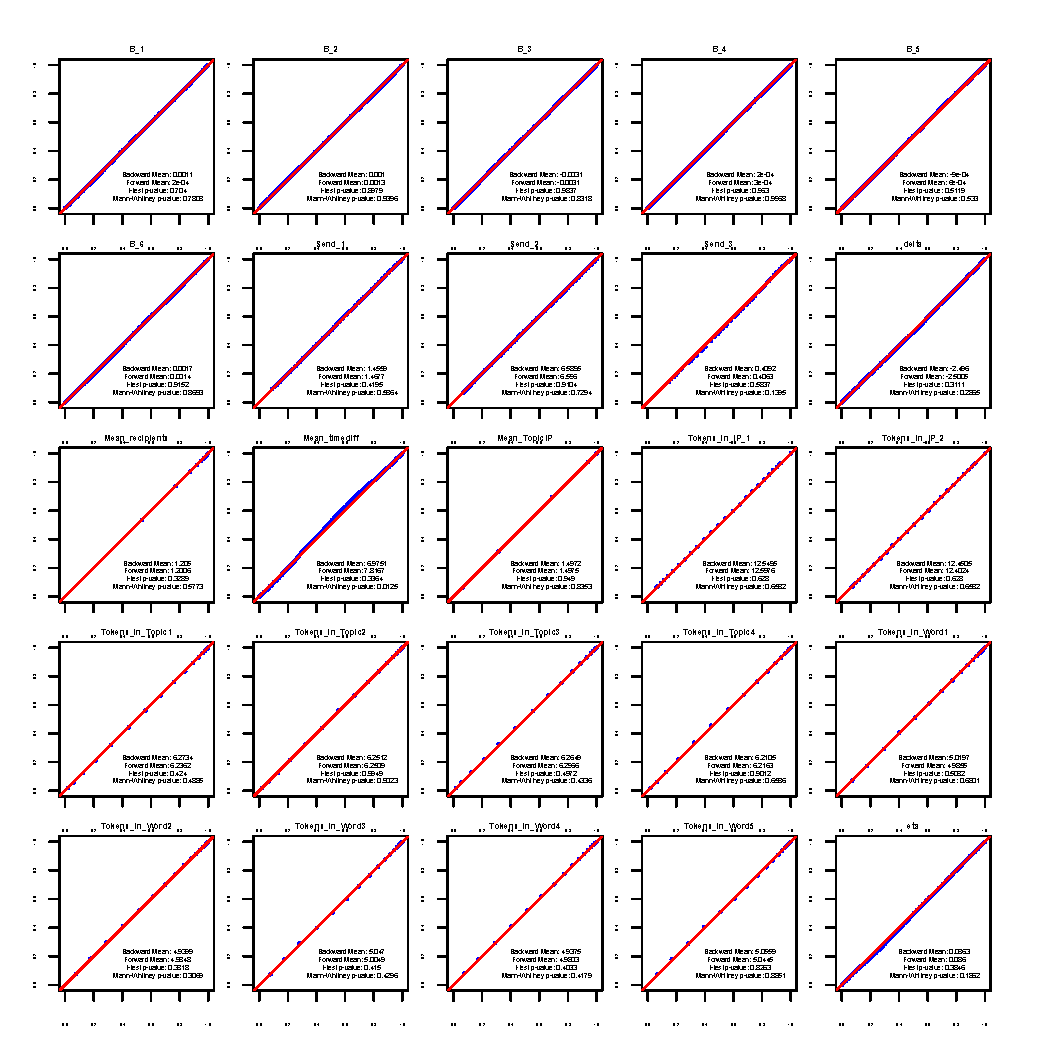
\includegraphics[width=1.1\textwidth]{plots/GiReta.pdf} 
	\label{fig:PPplot2}
	\caption{Probability-Probability plot for the 25 GiR test statistics.}
\end{figure}
\bibliographystyle{apalike}
\bibliography{IPTM}
\appendix
 \section*{Appendix}
 \renewcommand{\thesubsection}{\Alph{subsection}}
  \subsection{GiR Implementation Details} \label{subsec: GiR implementation}
  While we tried a number of different parameter combinations in the course of testing, we outline our standard setup. We selected the following parameter values:
  \begin{itemize}
  	\begin{minipage}{0.49\textwidth}
  		\item[-] $D$ (number of documents) = 5
  		\item[-] $N_d$ (tokens per document) = 6
  		\item[-] $A$ (number of actors)= 4
  		\item[-] $V$ (unique word types) = 5
  		\item[-] $C$ (number of interaction patterns) = 2
  		\item[-] $K$ (number of topics) = 4
  		\item[-] $\alpha$ (Dirichlet concentration prior) = 2
  		\item[-] $\boldsymbol{m}$ (Dirichlet base prior) = $(\frac{1}{K},\ldots, \frac{1}{K})$ 
  		\item[-] $\beta$ (Dirichlet concentration prior)= 2
  		\item[-] $\boldsymbol{n}$ (Dirichlet base prior) =$(\frac{1}{V},\ldots, \frac{1}{V})$ 
  		\item[-] netstat = ``intercept" and ``dyadic"
	   \item[-] timestat = ``timeofday" and ``dayofweek" 
  	\end{minipage}
  	\begin{minipage}{0.49\textwidth}
  		\item[-] prior for $\{\boldsymbol{b}_c\}_{c=1}^C$: $\mu_{\boldsymbol{b}} = \boldsymbol{0}_7, \Sigma_{\boldsymbol{b}} =  I_7$
  			\item[-] prior for $\{\boldsymbol{\eta}_c\}_{c=1}^C$: $\mu_{\boldsymbol{\eta}} = \boldsymbol{0}_7, \Sigma_{\boldsymbol{\eta}} =  I_7$
  		\item[-] prior for $\delta$: $\mu_\delta = -2.5$, $\sigma^2_\delta =0.1$
  		\item[-] prior for $\sigma^2_\tau$: $a_\tau = 1$, $b_\tau = 0.01$
  		\item[-] Outer (outer iteration) = 3
  		\item[-] Inner (M-H sampling iterations) = $(5500, 5500)$
  		\item[-] burn (M-H sampling burn-in)= (500, 500)
  		\item[-] thin (M-H sampling thinning)= (5, 5)
  		 \item[-] $n_1$ (hyperparamter optimization) = 0
  		\item[-] $\sigma_Q$ (proposal variance) = (0.01, 0.005)
  	\end{minipage}
  \end{itemize}        
        \subsection{Intitialization of History $\boldsymbol{x}$} \label{subsec: Initial history issue}
        Considering that our network statistics $\boldsymbol{x}$ are generated as a function of the network history, it is necessary to use the same initial value of $\boldsymbol{x}$ across the forward and backward samples. If not, when we generate fixed number of documents, we cannot guarantee the same number of documents used for the inference, since only the documents with its timestamp greater than 384 hours are used in the inference. In the extreme cases, we may end up with two types of failure:
        \begin{itemize}
        	\item[1.] Zero document generated after 384 hours (i.e. $t_{d=10}< 384$), making no documents to be used for inference,
        	\item[2.] Zero document generated before 384 hours (i.e. $t_{d=1}> 384$), making the estimates of $\boldsymbol{b}$ and $\boldsymbol{\eta}$ totally biased since $\forall  \boldsymbol{x}_{idjc} = 0$. 
        \end{itemize}
        Therefore, we fix the initial state of $\boldsymbol{x}$ over the entire GiR process. Specifically, we fix some baseline documents where the timestamps are all smaller than 384 and use as an input for forward sampling, backward sampling, and the inference. Then, in the forward and backward generative process, we set the starting point of the timestamp as $t_0= 384$ and generate fixed number of documents given the initial history or network statistics so that we can acheive consistency in the generated number of documents with $t_d > 384$.
  
  
    \subsection{Tips for GiR} \label{subsec: Tips for GiR}
    Schein test by set outer, inner the smallest (e.g. 1)  -> should pass unless significant bug in code   
                \end{document}

